\documentclass{article}
\usepackage{graphicx}
\usepackage[utf8]{inputenc}
\usepackage[T1]{fontenc}
\usepackage[francais]{babel}
\usepackage{layout}
\usepackage{caption}

\begin{document}
\begin{titlepage}
\begin{center}
\Huge Rapport TPA phase 1

\normalsize
\vspace{0.5cm}
\Large {\underline{ Groupe 3 Bleu : Sokoban} }

\vspace{1cm}

\normalsize
Goron Nathan, De La Rosa Louis-David, Basset Emilien, Demé Quentin

\vspace{1cm}
\begin{center}
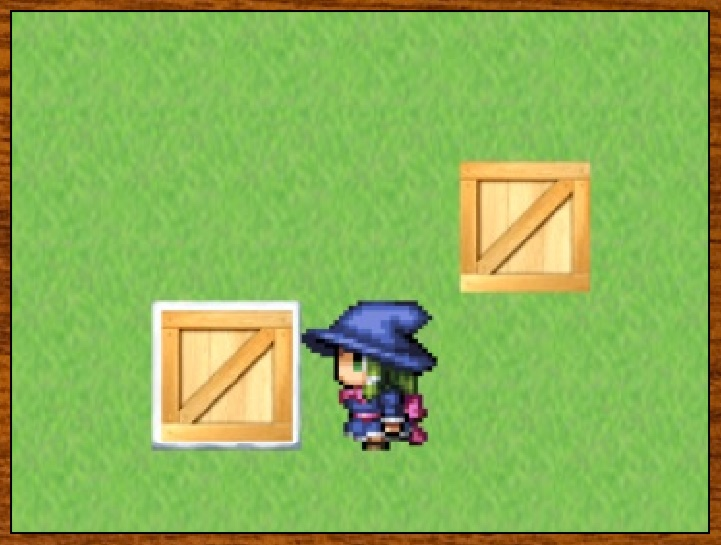
\includegraphics[scale=0.7]{../Screenshots/main.jpg}
\end{center}
\vspace{3.5cm}
L2 informatique 2016-2017 Université de Caen Basse-Normandie
\end{center}
\end{titlepage}


\newpage
\tableofcontents

\newpage
\begin{center}
	\section{Introduction}
\end{center}
\vspace{1cm}
	Parmi les projets proposés , nous avons fais le choix d'éviter les projets n'étant pas des jeux de peur qu'ils limitent notre créativité et notre motivation quant a son développement.Le jeu de Sokoban nous paraissait être un projet ambitieux et intéressant de par la difficulté dans l'implémentation de son IA.
 \vspace{0.5cm}

	Il s'agissait donc de développer un Jeu de Sokoban : Un jeu de puzzle dans lequel un personnage déplace un certains nombres de caisse sur des emplacements dans un niveau fermé ,le joueur gagne la partie si il parvient a boucher toutes les emplacements avec des caisses.
	
	Après avoir songé à l'utilisation de l'Unreal Development Kit(UDK) , nous avons décidé de développer ce projet en Python avec l'aide de la librairie PyGame qui offre une grande liberté dans l'interface graphique ainsi que de nombreuses méthodes facilitant les mécaniques de fonctionnement de base du jeu. 
	\newpage
	\begin{center}
	\section{Cahier de charges}
	\end{center}
	\vspace{1cm}
		\subsection{Déroulé fonctionnel , objectif}
		Le programme sera écrit en Python a l’aide de la librairie Pygame et répondra
au critères suivants d’ici la version finale de son développement :
			\subsubsection{Phase 1 :}
			-Le jeu sera jouable par humain via un prototype non-définitif(changements
possibles en phase2) , le joueur pourra se déplacer dans un niveau importé
au format .slc composé de plusieurs éléments expliqués dans les détails de fonctionnement du moteur de jeu.
			\subsubsection{Phase 2 :}
			Le jeu se verra ajouter une fonctionnalité de résolution automatique grâce
a l’algorithme A* et aux heuristiques, cet algorithme proposera un chemin optimal(dans
la plupart des cas en fonction de la difficulté)pour compléter le niveau
en le moins de coup possibles.Cet algorithme devra être anytime , càd capable
de compléter un niveau quelque soit son point de départ.
Les fonctionnalités additionnelles facultatives sont listées dans la catégorie
"Fonctionnalités additionnelles"
		\subsection{Contexte de réalisation}
		Ce projet est réalisé dans le cadre de l’évaluation de la valeur "TPA" en L2
info 2016-2017 de l’université de Caen
		\subsection{Découpage}
		Le programme sera composé des modules suivants :
— Le module sokoban qui assurera le fonctionnement général du programme
(moteur de jeu, conditions de victoire,interface graphique, importations
des niveaux)
— Le module classes qui comprendra toutes les classes et méthodes nécessaire
au fonctionnement du jeu
— Le module constantes stockant les importations d’images pour les personnages
et les cases ainsi que les variables nécessaire pour les variations
de tailles de niveaux a l’écran.
-Le module Sokobastar qui gérera le 
Ce découpage pourra être modifié en fonction des choix de fonctionnalités additionnelles
		\subsection{Pré-requis d'utilisation}
		Le jeu fonctionnera sous n’importe quel système muni de python(2.7 a 3.5) et
de la librairie Pygame. Le jeu sera intuitif d’utilisation et ne nécessitera aucune
connaissance informatique avancée particulière .
		\subsection{Règles du jeu}
		le joueur déplace un personnage dans un niveau constitué de murs , de cases
vides , de caisses et de socle pour les caisses.Il faudra déplacer les caisses dans
le niveau afin de couvrir tous les socles pour terminer le niveau. Le joueur peut
que pousser (pas tirer) , il ne peut pousser qu’une seule caisse a la fois. Le joueur
peut se retrouver bloqué
		\subsection{Fonctionnalité additionnelles}
			6 Fonctionnalité additionnelles :
Les fonctionnalités suivantes seront susceptible d’être implémentée d’ici la
version finale du programme :
— Menu permettant le choix du niveau et la modifications d’éventuelles
options(sons , design de la fenêtre...)
— Bouton "undo" permettant d’annuler le dernier mouvement du joueur
— Système de sauvegarde pour conserver son avancée dans un niveau
		\subsection{Calendrier , dates fixées}
		Le développement du jeu est découpé en deux phase :
-phase 1/1er semestre : réalisation d’un jeu jouable par un humain et recherches
sur l’IA (A* , heuristiques) , importation des niveaux
-phase 2/2nd semestre : programmation de la résolution automatique anytime et ajout d'éventuelles fonctionnalités additionnelles
		\subsection{Internationalité}
		8 Internationalité :
Le jeu ne sera pas traduit et sera utilisable uniquement en Français.
		\subsection{Priorités , importances relatives des fonctionnalités}
		Le fonctionnement du jeu sans IA et la possibilité d’importation des niveaux
sont prioritaires, la résolution automatique ne sera programmée qu’ensuite .Les
fonctionnalités additionnelles ne seront développées qu’une fois les objectifs des
deux phases remplies.
	\newpage
	\begin{center}
	\section{Détails du fonctionnement}
		\vspace{0.5cm}
		Pour des raisons de clarté et de facilitation d'implémentation , nous avons choisi d'implémenter notre programme en orienté objet plutôt qu'en procédural .
		\end{center}
		\vspace{0.5cm}
		\subsection{Moteur de jeu}
			Notre moteur de jeu repose sur 5 classes :
			\begin{itemize}
				\item Sprite 
				\item Personnage 
				\item Caisse
				\item Niveau
				\item LevelCollection
				\end{itemize}
				\vspace{0.5cm}
			Les classes Sprite , Personnage et Caisse servent a représenter visuellement les objets suivants:
				\begin{itemize}
					\item Le personnage - Il représente le personnage contrôlé par le joueur
					\item Les caisses - Les entités manipulable par le personnage
					\item Les murs - Moteur de difficulté du jeu ; Ils bloquent le déplacement des caisses et du personnage
					\item Les cibles - Emplacements sur lesquels il faut placer les caisses
					\item Les cases vides - Cases sur lesquels les personnage et caisses peuvent se déplacer
				\end{itemize}
				\vspace{0.5cm}
				Pour construire notre plan de jeu , nous avons choisi de décomposer notre niveau en 2 grilles nommées GameP et GameO contenant a elles deux les objets cités plus haut ; la grille gameP(game plan)contient les cibles et les espaces vides tandis que la grille gameO(game Obstacle) contient les murs , les caisses et le personnage
			\begin{figure}
			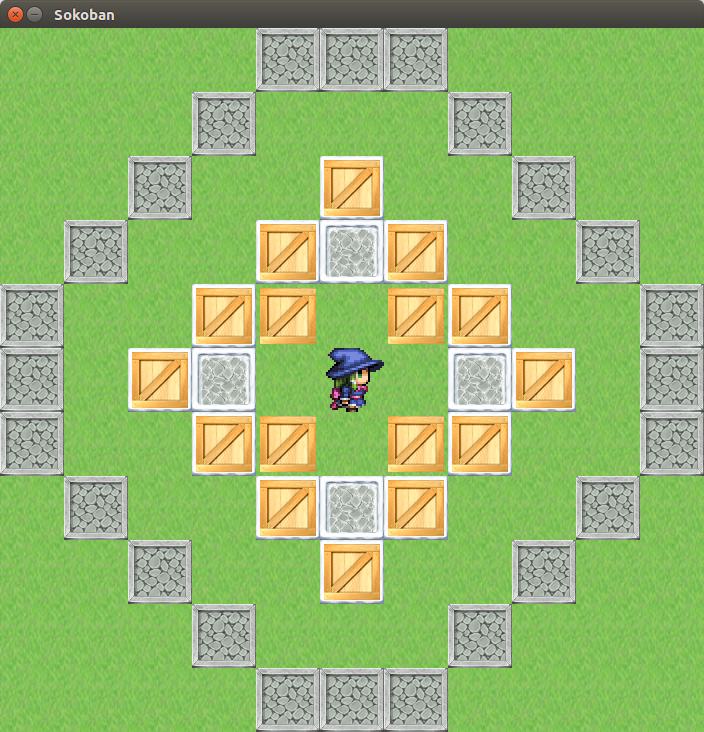
\includegraphics[width=.48\linewidth]{../Screenshots/05.png}
			\caption{sdfio}
			\includegraphics[width=.48\linewidth{../Screenshots/06.png}
			\caption{sdfio}
			\end{figure}
				
		\subsection{Astar}
		\newpage
	\section{Schéma UML}
	\newpage
	\section{Perspectives d'améliorations en phase 2}
	\newpage
	\section{Session de tests}
	\newpage
	\section{État du projet en fin de phase 1}
	\section{Résumé , conclusion de la phase 1}


		

\newpage
\end{document}